        %%******************************************%%
        %%                                          %%
        %%        Modello di tesi di laurea         %%
        %%            di Andrea Giraldin            %%
        %%                                          %%
        %%             2 novembre 2012              %%
        %%                                          %%
        %%******************************************%%

\begin{document}
    \frontmatter
    \begin{titlepage}
    \begin{center}
        \begin{LARGE}
            \textbf{\myUni}\\
        \end{LARGE}

        \vspace{10pt}

        \begin{Large}
            \textsc{\myDepartment}\\
        \end{Large}

        \vspace{10pt}

        \begin{large}
            \textsc{\myFaculty}\\
        \end{large}

        \vspace{30pt}
        \begin{figure}[htbp]
            \centering
            
\includegraphics[height=6cm]{unipd-logo}
        \end{figure}
        \vspace{30pt}

        \begin{LARGE}
            \textbf{\myTitle}\\
        \end{LARGE}

        \vspace{10pt}

        \begin{large}
            \textsl{\myDegree}\\
        \end{large}

        \vspace{40pt}

        \begin{large}
            \begin{flushleft}
                \textit{Relatore}\\
                \vspace{5pt}
                \profTitle\ \myProf
            \end{flushleft}

            % You can tweak the spacing to have professor and student names on the same line
            % useful if the page is broken by a long thesis title and you need more space
            % \vspace{-52pt}

            \begin{flushright}
                \textit{Laureando}\\
                \vspace{5pt}
                \myName \\
                \vspace{5pt}
                \textit{Matricola} \myID
            \end{flushright}
        \end{large}

        \vspace{40pt}

        \line(1, 0){338} \\
        \begin{normalsize}
            \textsc{Anno Accademico \myAA}
        \end{normalsize}
    \end{center}
\end{titlepage}

    \clearpage
\phantomsection
\thispagestyle{empty}

\hfill
\vfill

\noindent\myName: \textit{\myTitle,}
\myDegree,
\textcopyright\ \myTime.

    \cleardoublepage
\phantomsection
\thispagestyle{empty}
\pdfbookmark{Dedica}{Dedica}

\vspace*{3cm}

\begin{center}
    "Nami tu sei la mia speranza. In questo mondo dove il potere è tutto, anche se vengo ferita e umiliata, voglio ancora lottare, correre e vivere il più liberamente possibile! \newline Se la penso così è solo grazie a te" \\ \medskip
    --- Ragazzina dai capelli arancioni
\end{center}

\medskip

\begin{center}
    Dedicato a ...
\end{center}

    \cleardoublepage
\phantomsection
\pdfbookmark{Sommario}{Sommario}
\begingroup
\let\clearpage\relax
\let\cleardoublepage\relax
\let\cleardoublepage\relax

\chapter*{Sommario}

Il presente documento descrive il lavoro svolto durante il periodo di stage, della durata di circa trecentoventi ore, dal laureando Carmelo Russello presso l'azienda Var Group S.p.A.
Gli obbiettivi da raggiungere erano molteplici.\\
\begin{itemize}
\item In primo luogo era richiesto lo sviluppo di un sistema di testing automatizzato per l'analisi di sicurezza e compliance OWASP dei modelli di intelligenza artificiale, utilizzando lo strumento Gandalf Test.
\item In secondo luogo era richiesta l'implementazione di una dashboard web per la visualizzazione dei risultati dei test eseguiti.
\end{itemize}

%\vfill

%\selectlanguage{english}
%\pdfbookmark{Abstract}{Abstract}
%\chapter*{Abstract}

%\selectlanguage{italian}

\endgroup

\vfill

    \cleardoublepage
\phantomsection
\pdfbookmark{Ringraziamenti}{ringraziamenti}

\begin{flushright}{
    \slshape
    ``Life is really simple, but we insist on making it complicated''} \\
    \medskip
    --- Confucius
\end{flushright}


\bigskip

\begingroup
\let\clearpage\relax
\let\cleardoublepage\relax
\let\cleardoublepage\relax

\chapter*{Ringraziamenti}

\noindent \textit{Innanzitutto, vorrei esprimere la mia gratitudine al Prof. \myProf, relatore della mia tesi, per l'aiuto e il sostegno fornitomi durante la stesura del lavoro.}\\

\noindent \textit{Desidero ringraziare con affetto i miei genitori per il sostegno, il grande aiuto e per essermi stati vicini in ogni momento durante gli anni di studio.}\\

\noindent \textit{Ho desiderio di ringraziare poi i miei amici per tutti i bellissimi anni passati insieme e le mille avventure vissute.}\\
\bigskip

\noindent\textit{\myLocation, \myTime}
\hfill \myName

\endgroup

    \cleardoublepage
\pdfbookmark{\contentsname}{tableofcontents}
\setcounter{tocdepth}{2}
\tableofcontents
%\markboth{\contentsname}{\contentsname}
\clearpage

\begingroup
    \let\clearpage\relax
    \let\cleardoublepage\relax
    \let\cleardoublepage\relax

    % Figures list
    \phantomsection
    \pdfbookmark{\listfigurename}{lof}
    \listoffigures

    \vspace*{8ex}

    % Tables list
    \phantomsection
    \pdfbookmark{\listtablename}{lot}
    \listoftables

    \vspace*{8ex}
\endgroup

\cleardoublepage

    \cleardoublepage

    \mainmatter
    \chapter{Introduzione}
\label{cap:introduzione}

Il presente capitolo introduce il contesto applicativo oggetto dello stage: automazione di testing su applicazioni che sfruttano l'intelligenza artificiale generativa, come chatbot o assistenti virtuali. Queste applicazioni trattano input testuali e informazioni sensibili, esponendo a rischi generali quali manipolazioni degli input, fuoriuscite di dati e comportamenti imprevisti dei modelli.\\
Il progetto mira a definire e implementare un approccio integrato per valutare e migliorare la sicurezza, l'affidabilità e la conformità delle applicazioni, attraverso analisi del codice, test e pratiche operative dedicate.\\
% \gls{api}. \\

% \noindent Esempio di citazione in linea \\
% \cite{site:agile-manifesto}. \\

% \noindent Esempio di citazione nel pie' di pagina \\
% citazione\footcite{womak:lean-thinking} \\

\section{L'azienda}
L'azienda con cui ho deciso di intraprendere il mio percorso di Stage è Var Group S.p.A., 
una realtà italiana specializzata in soluzioni IT e servizi di consulenza per le imprese.\\
La scelta è stata influenzata dalla mia precedente esperienza con il progetto di Software Engineering svolto presso Var Group,
durante il quale ho avuto modo di apprezzare la professionalità e la competenza del team.

\section{L'idea}
Il progetto di stage è incentrato sulla sicurezza delle applicazioni basate su AI generativa, con particolare attenzione all'impiego di analisi statica e dinamica del codice per verificarne la conformità alle linee guida OWASP. \\
L'obiettivo è sviluppare un sistema di testing e verifica capace di rilevare e prevenire vulnerabilità specifiche (come le tecniche di prompt injection) evitando la divulgazione di informazioni riservate a utenti non autorizzati e impedendo l'introduzione di falle nell'applicativo.\\
Il lavoro comprende inoltre la progettazione e l'integrazione di workflow e strumenti automatizzati per l'analisi del flusso dei dati, il fuzzing e i penetration test, nonché la definizione di procedure di mitigazione e di reporting delle vulnerabilità individuate.


Riguardo la stesura del testo, relativamente al documento sono state adottate le seguenti convenzioni tipografiche:
\begin{itemize}
	\item gli acronimi, le abbreviazioni e i termini ambigui o di uso non comune menzionati vengono definiti nel glossario, situato alla fine del presente documento;
	\item per la prima occorrenza dei termini riportati nel glossario viene utilizzata la seguente nomenclatura: \emph{parola}\glsfirstoccur;
	\item i termini in lingua straniera o facenti parti del gergo tecnico sono evidenziati con il carattere \emph{corsivo}.
\end{itemize}

    \chapter{Processi e metodologie}
\label{cap:processi-metodologie}

\intro{Brevissima introduzione al capitolo}\\

\section{Processo sviluppo prodotto}

    \chapter{Descrizione dello stage}
\label{cap:descrizione-stage}

\intro{Breve introduzione al capitolo}\\

\section{Introduzione al progetto}


\section{Analisi preventiva dei rischi}

Durante la fase di analisi iniziale sono stati individuati alcuni possibili rischi a cui si potrà andare incontro.
Si è quindi proceduto a elaborare delle possibili soluzioni per far fronte a tali rischi.\\

\subsection{Rischi tecnici}

\begin{risk}{Complessità nell'applicare strumenti di security testing ad AI generativa (tool immaturi o
non sempre affidabili).}
    \riskdescription{le performance del simulatore hardware e la comunicazione con questo potrebbero risultare lenti o non abbastanza buoni da causare il fallimento dei test}
    \risksolution{coinvolgimento del responsabile a capo del progetto relativo il simulatore hardware}
\end{risk}

\begin{risk}{Possibili falsi positivi o negativi nei test di vulnerabilità.}
    \riskdescription{le performance del simulatore hardware e la comunicazione con questo potrebbero risultare lenti o non abbastanza buoni da causare il fallimento dei test}
    \risksolution{coinvolgimento del responsabile a capo del progetto relativo il simulatore hardware}
\end{risk}

\begin{risk}{Difficoltà di integrazione dei tool con codice reale e pipeline di sviluppo.}
    \riskdescription{le performance del simulatore hardware e la comunicazione con questo potrebbero risultare lenti o non abbastanza buoni da causare il fallimento dei test}
    \risksolution{coinvolgimento del responsabile a capo del progetto relativo il simulatore hardware}
\end{risk}

\subsection{Rischi di progetto}

\begin{risk}{Mancanza di esperienza pregressa su OWASP o sicurezza AI.}
    \riskdescription{le performance del simulatore hardware e la comunicazione con questo potrebbero risultare lenti o non abbastanza buoni da causare il fallimento dei test}
    \risksolution{coinvolgimento del responsabile a capo del progetto relativo il simulatore hardware}
\end{risk}

\begin{risk}{Possibile difficoltà a rispettare la pianificazione a causa della curva di apprendimento iniziale.}
    \riskdescription{le performance del simulatore hardware e la comunicazione con questo potrebbero risultare lenti o non abbastanza buoni da causare il fallimento dei test}
    \risksolution{coinvolgimento del responsabile a capo del progetto relativo il simulatore hardware}
\end{risk}

\subsection{Rischi infrastrutturali}

\begin{risk}{Limitazioni di risorse computazionali nei test di AI.}
    \riskdescription{le performance del simulatore hardware e la comunicazione con questo potrebbero risultare lenti o non abbastanza buoni da causare il fallimento dei test}
    \risksolution{coinvolgimento del responsabile a capo del progetto relativo il simulatore hardware}
\end{risk}

\begin{risk}{Problemi di compatibilità con ambienti cloud o di deployment.}
    \riskdescription{le performance del simulatore hardware e la comunicazione con questo potrebbero risultare lenti o non abbastanza buoni da causare il fallimento dei test}
    \risksolution{coinvolgimento del responsabile a capo del progetto relativo il simulatore hardware}
\end{risk}


\section{Requisiti e obiettivi}


\subsection{Obiettivi obbligatori}
\begin{itemize}
\item Valutazione comparativa degli strumenti di analisi.
\item Applicazione pratica dei test su codice reale.
\item Prototipo in grado di generare report sulle vulnerabilità AI rispetto a OWASP.
\item Documentazione tecnica e presentazione finale.
\end{itemize}

\subsection{Obiettivi desiderabili}
\begin{itemize}
\item Dashboard interattiva con visualizzazioni avanzate
\item Integrazione del prototipo in pipeline CI/CD esistente.
\item Estensione dei test ad altri framework oltre Gandalf Test.
\item Raccomandazioni per un framework interno di AI Security by Design.
\end{itemize}

\section{Pianificazione}

La pianificazione del lavoro di progetto è stata suddivisa in fasi settimanali, con obiettivi specifici per ciascuna fase. Di seguito è riportata una panoramica della pianificazione prevista:

\begin{table}[htbp]
    \centering
    \renewcommand{\arraystretch}{1.2}
    \begin{tabular}{|p{3cm}|p{10cm}|}
        \hline
        \textbf{Settimana} & \textbf{Attività} \\
        \hline
        Settimana 1 & Studio preliminare su OWASP e rischi AI, overview di Gandalf Test, setup ambiente di
lavoro.\\
        \hline
        Settimana 2 & Analisi comparativa di tool di analisi statica e dinamica (open-source e commerciali).
Creazione matrice di valutazione.\\
        \hline
        Settimana 3 & Applicazione degli strumenti a piccoli progetti demo, valutazione dei risultati e raccolta
criticità.\\
        \hline
        Settimana 4 & Esecuzione dei primi test su componenti reali del team, documentazione dei risultati,
identificazione vulnerabilità.\\
        \hline
        Settimana 5 & Realizzazione di script/report per aggregare risultati, definizione dei KPI di compliance
OWASP.\\
        \hline
        Settimana 6 & Sviluppo di dashboard interattiva per monitorare vulnerabilità e andamento dei test.\\
        \hline
        Settimana 7 & Test end-to-end sul prototipo, miglioramento dei tool e dei report.\newline\mbox{}\\
        \hline
        Settimana 8 & Redazione di documentazione tecnica, manuale utente e materiale per la presentazione
della tesi.\\
        \hline
    \end{tabular}
    \caption{Pianificazione delle attività di progetto}
\end{table}
    \chapter{Analisi dei requisiti}
\label{cap:analisi-requisiti}

\intro{Breve introduzione al capitolo}\\

\section{Casi d'uso}

Per lo studio dei casi di utilizzo del prodotto sono stati creati dei diagrammi.
I diagrammi dei casi d'uso (in inglese \emph{Use Case Diagram}) sono diagrammi di tipo \gls{uml} dedicati alla descrizione delle funzioni o servizi offerti da un sistema, così come sono percepiti e utilizzati dagli attori che interagiscono col sistema stesso.
Essendo il progetto finalizzato alla creazione di un tool per l'automazione di un processo, le interazioni da parte dell'utilizzatore devono essere ovviamente ridotte allo stretto necessario. Per questo motivo i diagrammi d'uso risultano semplici e in numero ridotto.

\begin{figure}[!h] 
    \centering 
    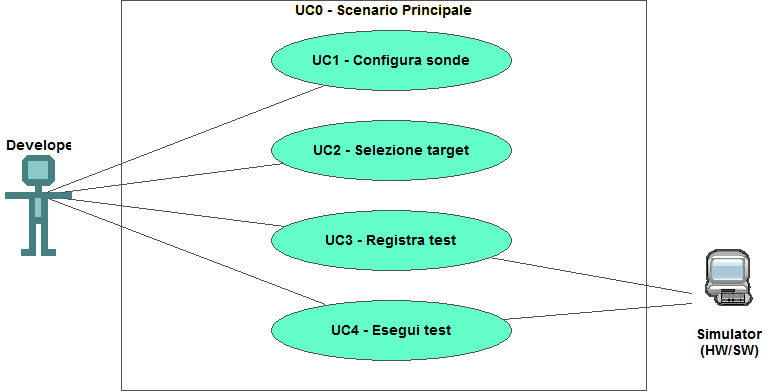
\includegraphics[width=0.9\columnwidth]{usecase/scenario-principale} 
    \caption{Use Case - UC0: Scenario principale}
\end{figure}

\begin{usecase}{0}{Scenario principale}
\usecaseactors{Sviluppatore applicativi}
\usecasepre{Lo sviluppatore è entrato nel plug-in di simulazione all'interno dell'IDE}
\usecasedesc{La finestra di simulazione mette a disposizione i comandi per configurare, registrare o eseguire un test}
\usecasepost{Il sistema è pronto per permettere una nuova interazione}
\label{uc:scenario-principale}
\end{usecase}

\section{Tracciamento dei requisiti}

Da un'attenta analisi dei requisiti e degli use case effettuata sul progetto è stata stilata la tabella che traccia i requisiti in rapporto agli use case.\\
Sono stati individuati diversi tipi di requisiti e si è quindi fatto utilizzo di un codice identificativo per distinguerli.\\
Il codice dei requisiti è così strutturato R(F/Q/V)(N/D/O) dove:
\begin{enumerate}
	\item[R =] requisito
    \item[F =] funzionale
    \item[Q =] qualitativo
    \item[V =] di vincolo
    \item[N =] obbligatorio (necessario)
    \item[D =] desiderabile
    \item[O =] opzionale
\end{enumerate}
Nelle tabelle \ref{tab:requisiti-funzionali}, \ref{tab:requisiti-qualitativi} e \ref{tab:requisiti-vincolo} sono riassunti i requisiti e il loro tracciamento con gli use case delineati in fase di analisi.

\newpage

\begin{table}%
\caption{Tabella del tracciamento dei requisti funzionali}
\label{tab:requisiti-funzionali}
\begin{tabularx}{\textwidth}{lXl}
\hline\hline
\textbf{Requisito} & \textbf{Descrizione} & \textbf{Use Case}\\
\hline
RFN-1     & L'interfaccia permette di configurare il tipo di sonde del test & UC1 \\
\hline
\end{tabularx}
\end{table}%

\begin{table}%
\caption{Tabella del tracciamento dei requisiti qualitativi}
\label{tab:requisiti-qualitativi}
\begin{tabularx}{\textwidth}{lXl}
\hline\hline
\textbf{Requisito} & \textbf{Descrizione} & \textbf{Use Case}\\
\hline
RQD-1    & Le prestazioni del simulatore hardware deve garantire la giusta esecuzione dei test e non la generazione di falsi negativi & - \\
\hline
\end{tabularx}
\end{table}%

\begin{table}%
\caption{Tabella del tracciamento dei requisiti di vincolo}
\label{tab:requisiti-vincolo}
\begin{tabularx}{\textwidth}{lXl}
\hline\hline
\textbf{Requisito} & \textbf{Descrizione} & \textbf{Use Case}\\
\hline
RVO-1    & La libreria per l'esecuzione dei test automatici deve essere riutilizzabile & - \\
\hline
\end{tabularx}
\end{table}%

    \chapter{Progettazione e codifica}
\label{cap:progettazione-codifica}

\intro{In questo capitolo }\\

\section{Tecnologie e strumenti}
\label{sec:tecnologie-strumenti}

Di seguito viene data una panoramica delle tecnologie e strumenti presi in considerazione per lo sviluppo del prototipo. L'analisi ha valutato compatibilità, licenza, facilità d'integrazione, costi e capacità di security testing specifiche per modelli generativi. Gli strumenti e le tecnologie esaminate includono:

\begin{itemize}
    \item \textbf{PromptFoo} -- piattaforma di testing per LLM con supporto a test automatizzati e integrazione CI/CD.
    \item \textbf{PyRIT} -- tool open-source per l'identificazione e mitigazione dei rischi sui modelli generativi.
    \item \textbf{LangFuse} -- piattaforma di osservabilità e valutazione di LLM.
    \item \textbf{DeepEval / DeepTeam} -- framework di valutazione e tool di red teaming per benchmark e safety testing.
    \item \textbf{Garak} -- scanner di vulnerabilità per modelli generativi focalizzato su attacchi pratici (prompt injection, jailbreak, leakage).
    \item \textbf{Giskard} -- piattaforma di red teaming automatizzato con opzioni SaaS e libreria Python.
    \item \textbf{Galileo} -- piattaforma di osservabilità con SDK, utile per monitoraggio ma meno orientata al security testing.
    \item \textbf{LakeraGuard} -- suite di sicurezza commerciale per modelli, include test come il Gandalf test.
    \item \textbf{Tecnologie di base} -- Python, Docker, Git/GitHub, CI/CD (GitHub Actions), librerie ML (PyTorch, Hugging Face), e strumenti di logging/monitoring.
\end{itemize}

Questa panoramica ha guidato la selezione degli strumenti adottati per il prototipo, privilegiando soluzioni open-source facilmente integrabili nell'ambiente di sviluppo e con funzionalità mirate al security testing dei modelli generativi.

\subsection{Strumenti analizzati}
Durante le prime due settimane di Stage è stato condotto uno studio preliminare su diversi strumenti di security testing per AI generativa. Di seguito viene fornita la matrice di valutazione dei tools e una breve descrizione di ciascuno strumento analizzato.

\begin{figure}[!h]
    \centering
    % includegraphics is redefined in config/thesis-config.tex to prepend
    % the images/ folder, so here we only pass the filename
    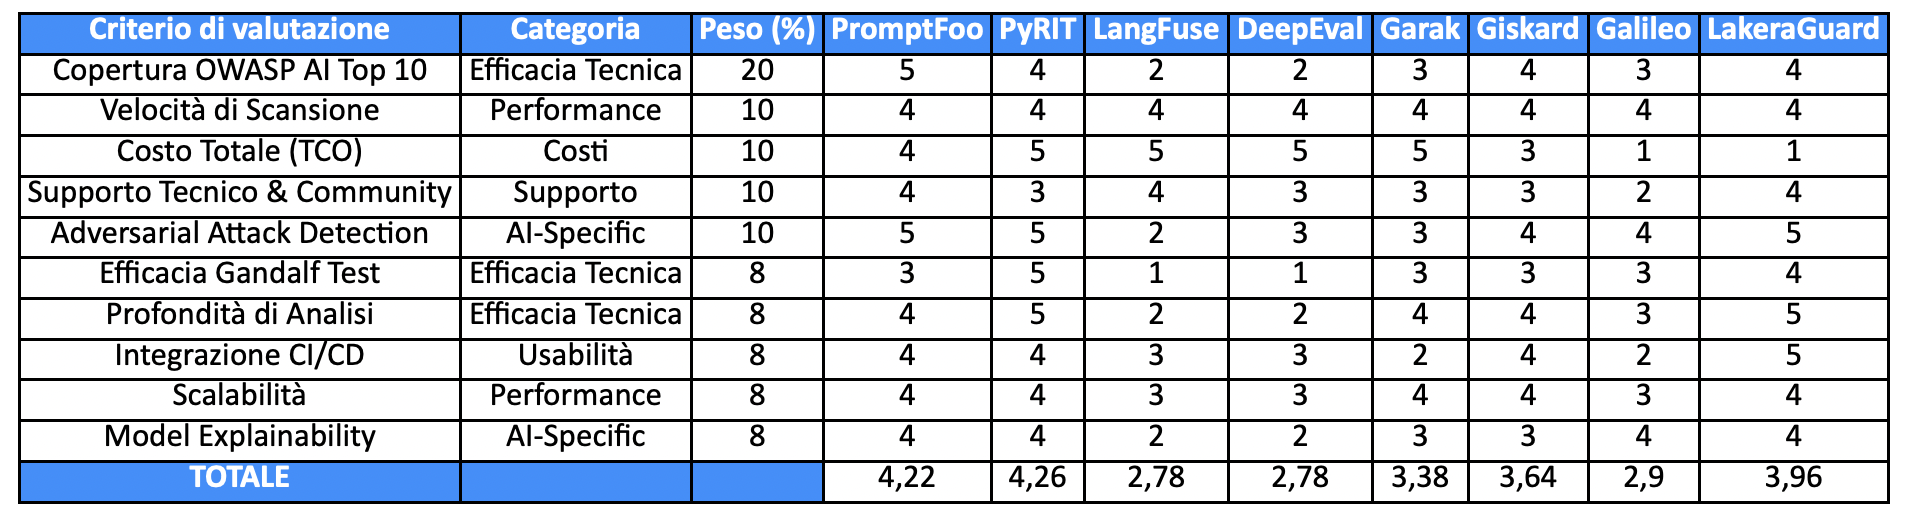
\includegraphics[width=1.0\columnwidth]{matrix.png}
    \caption{Matrice di Valutazione degli Strumenti Analizzati}
\end{figure}

\subsubsection*{PromptFoo}
PromptFoo è una piattaforma di testing per modelli di linguaggio che consente agli sviluppatori di creare, eseguire e gestire test automatizzati per valutare le prestazioni, l'affidabilità e la sicurezza dei loro modelli di linguaggio naturale. Offre funzionalità come la creazione di casi di test personalizzati, l'integrazione con pipeline CI/CD e report dettagliati sui risultati dei test.
Questo tool è stato tenuto in molta considerazione in quanto offre funzionalità specifiche per il testing delle vulnerabilità OWASP top 10 per AI generativa, obbiettivo principale del progetto di stage.

\subsubsection*{PyRIT}
PyRIT è uno tool open-source progettato da Azure Microsoft per l'identificazione e la mitigazione dei rischi associati all'uso di modelli di intelligenza artificiale generativa. PyRIT è stato creato per valutare modelli di AI per potenziali vulnerabilità di sicurezza, bias e problemi di conformità, fornendo raccomandazioni su come migliorare la sicurezza e l'affidabilità dei modelli.\\


\subsubsection*{LangFuse}
LangFuse è una piattaforma open-source per la valutazione e l'osservazione delle applicazioni che utilizzano intelligenza artificiale generativa. La piattaforma è integrata con diversi modelli di linguaggio naturale e permette l'utilizzo tramite cloud o in self host. Langfuse offre inoltre un LLM playground per testatre i modelli che aveva catturato la mia attenzione all'inizio del progetto. Tuttavia il tool non offre una vera e propria funzionalità di security testing, focus del progetto di stage.

\subsubsection*{DeepEval / DeepTeam}
DeepEval è un framework open-source per la valutazione e il benchmarking dei modelli di intelligenza artificiale generativa. DeepEval non fornisce funzionalità specifiche per il testing dei modelli. Per ovviare a questa mancanza è stato creato un tool di testing basato su DeepEval chiamato DeepTeam, un tool di red teaming. Tuttavia, DeepTeam non ha un focus sulle vulnerabilità OWASP in quanto si concentra sul testing delle safety guidelines.

\subsubsection*{Garak}
Garak è uno scanner di vulnerabilità per modelli di intelligenza artificiale generativa open-source creato da NVIDIA per facilitare il testing dei modelli. Il focus di Garak sta nei metodi di attacco specifici per far fallire in modo imprevisto una LLM o un sistema di dialogo. Garak testa diverse vulnerabilità tra cui allucinazioni, data leakage, prompt injection, jailbreaks ecc.

\subsubsection*{Giskard}
Giskard è una piattaforma di red teaming automatizzato per testare, valutare ed analizzare modelli di intelligenza artificiale generativa. Esistono due metodi di utilizzo di Giskard: Come servizio HUB a pagamento o come libreria Python open-source da installare localmente. La libreria fornita è però fortemente limitata nelle funzionalità rispetto al servizio HUB in quanto incentrata sulla ricerca.

\subsubsection*{Galileo}
Galileo è una piattaforma che permette la valutazione e osservazione di applicazioni basate su AI generativa. Galileo offre SDK in Python e TypeScript per integrarlo direttamente nei propri progetti. Galileo è molto flessibile per quanto riguarda il deploy e viene utilizzato da molte aziende di rilievo. Nonostante ciò la piattaforma non offre funzionalità specifiche per il security testing, focus di questo progetto, ed è a pagamento.

\subsubsection*{LakeraGuard}
LakeraGuard è una piattaforma di sicurezza per modelli di intelligenza artificiale che aiuta gli sviluppatori a proteggere i loro modelli da minacce e vulnerabilità. Offre funzionalità come la scansione delle vulnerabilità, la gestione delle patch e il monitoraggio delle minacce in tempo reale.\\
Essendo l'azienda svizzera Lakera la creatrice del gandalf test, focus principale delle prime settimane del progetto di stage, il tool da loro creato è stato uno dei primi ad essere analizzato. 
Tuttavia il tool out of the box fa già quello che lo stage chiede di implementare quindi non ha suscitato uno studio approfondito in quanto avrebbe reso superfluo lo sviluppo del prototipo.\\
Inoltre è un tool a pagamento che offre un tier gratuito il quale è però limitato a 10000~richieste \gls{api} al mese, limite che avrebbe reso difficile l'utilizzo futuro del tool.


\subsection{Strumenti utilizzati}
Di seguito viene data una panoramica delle tecnologie e strumenti utilizzati per lo sviluppo del prototipo.

\subsubsection*{Python + PyRIT (backend)}
Python è un linguaggio di programmazione versatile e ampiamente utilizzato, particolarmente adatto per lo sviluppo di applicazioni backend. PyRIT è uno strumento open-source progettato da Azure Microsoft per l'identificazione e la mitigazione dei rischi associati all'uso di modelli di intelligenza artificiale generativa. Insieme, Python e PyRIT forniscono un ambiente potente per lo sviluppo e la sicurezza delle applicazioni AI.DA AGGIUNGERE PERCHÉ USATO

\subsubsection*{React (frontend)}
React è una libreria JavaScript per la creazione di interfacce utente, sviluppata da Facebook. È ampiamente utilizzata per costruire applicazioni web dinamiche e reattive. La sua architettura basata su componenti consente agli sviluppatori di creare interfacce utente modulari e riutilizzabili, semplificando il processo di sviluppo.DA AGGIUNGERE PERCHÉ USATO

\subsubsection*{MongoDB (persistenza dati)}
MongoDB è un database NoSQL orientato ai documenti, progettato per gestire grandi volumi di dati non strutturati. Utilizza un modello di dati flessibile basato su JSON, che consente agli sviluppatori di archiviare e recuperare informazioni in modo efficiente. MongoDB è particolarmente adatto per applicazioni che richiedono scalabilità e prestazioni elevate.DA AGGIUNGERE PERCHÉ USATO

\section{Ciclo di vita del software}
\label{sec:ciclo-vita-software}

\section{Progettazione}
\label{sec:progettazione}

\subsubsection{Namespace 1} %**************************
Descrizione namespace 1.

\begin{namespacedesc}
    \classdesc{Classe 1}{Descrizione classe 1}
    \classdesc{Classe 2}{Descrizione classe 2}
\end{namespacedesc}


\section{Design Pattern utilizzati}

\section{Codifica}

    \chapter{Conclusioni}
\label{cap:conclusioni}

\section{Consuntivo finale}

\section{Raggiungimento degli obiettivi}

\section{Conoscenze acquisite}

\section{Valutazione personale}


    \appendix
    \chapter{Appendice A}

\epigraph{Citazione}{Autore della citazione}


    \backmatter
    % Ensure all glossary entries are included even if not referenced in the text
    \glsaddall
    % Also include all acronyms even if not used explicitly
    \glsaddall[types=\acronymtype]
    \printglossary[type=\acronymtype, title=Acronimi e abbreviazioni, toctitle=Acronimi e abbreviazioni]
    \printglossary[type=main, title=Glossario, toctitle=Glossario]

    \cleardoublepage
\chapter{Bibliografia}

\nocite{*}

% Print book bibliography
\printbibliography[heading=subbibliography,title={Riferimenti bibliografici},type=book]

% Print site bibliography
\printbibliography[heading=subbibliography,title={Siti web consultati},type=online]

\end{document}
